\aufgabenstellung{Schreiben Sie ein ein­fach­es Pro­gramm, das eine sortierte 
Liste der in einem 
Text vork­om­menden Worte (im weitesten Sinn alles was durch Leerze­ichen 
be­gren­zt wird) mit den as­sozi­ierten Häufigkeit­en (ab­so­lut und 
prozen­tu­al) er­stellt und sortiert ausgibt. (2 Punk­te)

    Ver­gle­ichen Sie an­hand der Aus­gabe Ihres Pro­gramms die 30 am 
häufig­sten vork­om­menden Worte in zwei oder mehreren längeren Tex­ten der 
gle­ichen Sprache (z. B. E-books, Pro­jekt Guten­berg, etc. ). Wählen Sie 
einge geeignete Darstel­lung für Ihren Ver­gle­ich.
    Sind diese Worte als Merk­male für Text-Klas­si­fizierungs-Auf­gaben 
geeignet? Warum?
    Mod­i­fizieren Sie Ihr Pro­gramm dahinge­hend, daß es eine Liste von 
Stop­pwörtern er­hal­ten kann, die ig­nori­ert werden. Wieder­holen Sie die 
vorherige Auf­gabe, indem Sie je­doch dies­mal die Stop­pwörter der 
jew­eili­gen 
Sprache ig­nori­eren (eine Auswahl find­en Sie unter 
\url{http://www.nltk.org/nltk_data/packages/corpora/stopwords.zip}
%​www.​nltk.​org/​nltk\_­da­ta/pack­ages/cor­po­ra/stopwords.​zip }
).
    Wie würden Sie nun die Eig­nung der 30 häufig­sten Wörter ein­schätzen?\\}
\loesung{Als zu vergleichende Texte wurden \textit{Frankenstein} von Mary 
Shelley und \textit{Die Verwandlung} von Franz Kafka in der englischen 
Übersetzung gewählt. Beide Werke wurden als Textdatei vom Projekt Gutenberg 
bezogen. Generische Textpassagen, die beispielweise Lizenzinformationen 
beinhalten wurden manuell entfernt.\\
Beim Betrachten der Liste (Abb. \ref{nostopwords}) fällt auf, dass die 30 häufigsten Wörter beider Texte zum größten Teil Pronomen (wie \textit{I}, \textit{he} oder \textit{you}) oder Konjunktionen (\textit{and}, \textit{for}) und Artikel (\textit{the}) sind. Da sich diese Wörter in quasi jedem englischen Text finden, sind sie nahezu bedeutungslos im Sinne der Text-Klassifizierung. Nur durch Kenntnis dieser Wörter ist es praktisch unmöglich, Rückschlüsse auf den Inhalt des Textes zu ziehen.\\
\begin{figure}[ht]
\begin{center}
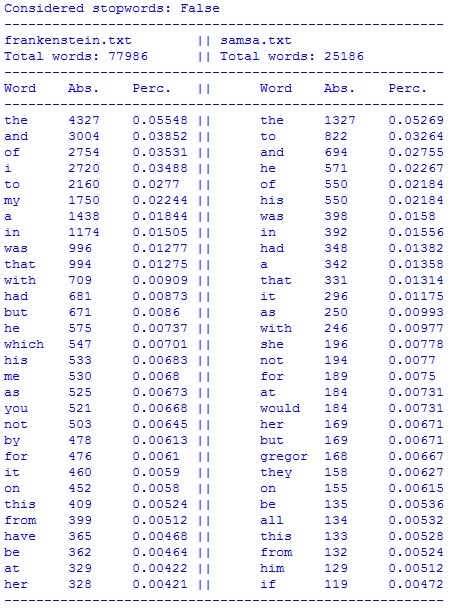
\includegraphics[width=0.8\textwidth]{img/false}
\caption{Liste der 30 am häufigsten vorkommenden Wörter in Frankenstein und Die Verwandlung}
\label{nostopwords}
\end{center}
\end{figure}
Die Einbeziehung einer Liste mit Stopwords soll genau solche Fälle verhindern. In einer solchen Liste sind Wörter enthalten, die keinerlei Aussagekraft über den Inhalt des Textes liefern und deshalb bei der Analyse außen vor gelassen werden sollen. Unter Nichtbeachtung dieser Wörter stellen sich die 30 häufigsten Wörter beider Texte wie in Abb. \ref{stopwords} dar.\\
\begin{figure}[ht]
\begin{center}
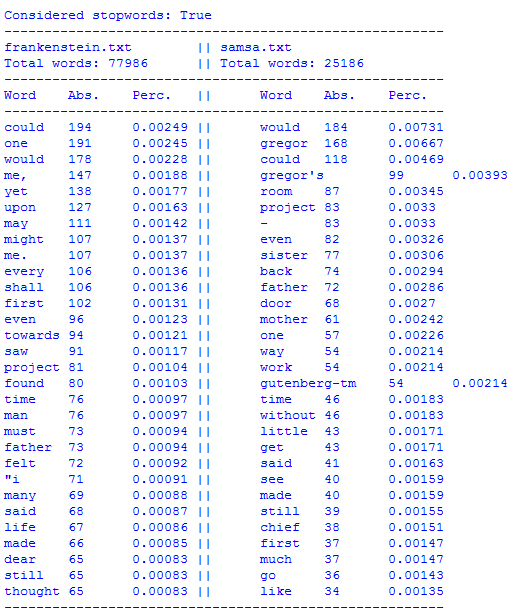
\includegraphics[width=0.8\textwidth]{img/true}
\caption{Liste der 30 am häufigsten vorkommenden Wörter in Frankenstein und Die Verwandlung unter Nichtbeachtung von Stopwords}
\label{stopwords}
\end{center}
\end{figure}
Nun befinden sich unter den 30 Wörtern auch solche, die zumindest grob Rückschlüsse auf den Inhalt der Texte zulassen, wie z. B. \textit{saw}, \textit{time}, \textit{father} (Frankenstein) oder \textit{gregor}, \textit{room}, \textit{sister} (Die Verwandlung).


}